\documentclass{article}
\usepackage{amsthm}
\usepackage{amsmath}
\usepackage{graphicx}

\newtheorem{problem}{Problem}

\begin{document}
\title{Hashing}
\author{Henry Z. Lo}
\maketitle

\section{Hash Tables}

\begin{problem}
Assume we have infinite memory.  What is the fastest way to sort a set of \textbf{unique} integers?  Having empty elements in the array is acceptable, as long as all non-empty elements are in order.
\end{problem}

$O(n)$!  We can use a form of bucket sort:

\begin{enumerate}
\item Create an infinite array of \verb|int|s, \verb|myArray|.
\item Loop through all the integers in our set.
\item Use each integer as an index to store itself.
\end{enumerate}

Admittedly, this is somewhat contrived.  But this illustrates the idea behind hashing: the idea being that in order to store an object, you can use that object itself as an index into an array (or any other data structure).

At some level, though, an index \textit{must} be an \verb|int|.  In our example, our objects are \verb|ints|, but we can generalize this to any type of object.  Converting that object to an \verb|int| is the job of a \textit{hash function}.  This type of data structure is a \textit{hash table}.

\begin{figure}
\centering
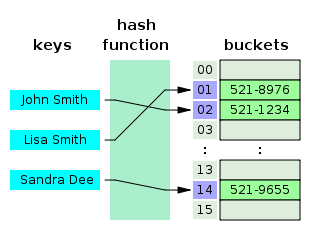
\includegraphics[scale=0.6]{img/hashtable.png}
\caption{A hash table.  In this case, we are hashing Objects containing names and phone numbers.  This example uses names as keys.}
\end{figure}

\subsection{Motivation}
Why bother with hash tables?  Constant time lookups.  Hash tables are one of the very few (the only?) data structures which allow looking up \textit{any} element, and checking membership of an element, in one operation.  Think about the other data structures you have learned, and how many computations a lookup takes on average.

\begin{enumerate}
\item Linked lists, arrays, stacks, etc.: on average $\frac{1}{2}n$ operations for lookup, where $n$ is the number of elements in the data structure
\item Balanced binary tree, binary search: on average $\log_2 (n) - 1$ operations.
\item Hash tables: on average one operation.
\end{enumerate}

If we consider checking elements which do not exist, the lookup time for all other data structures is even slower.  For hash tables, it still only takes one operation.

\subsection{Architecture}

You may have already guessed how this magical hash table works.  For sake of implementation, let's say the table is an array.  A hash function is any function that turns an object into an index; we can be general about this.

If we have an object $o$, a table $t$, and a hash function $f$, then we just do the following for a lookup:

\begin{enumerate}
\item Convert $o$ (or part of $o$, which we call the $key$) into an index using $f$
\item Look up the index in the table, e.g. $t[f(o)]$
\item If there is something there, return it.
\end{enumerate}

We have already discussed inserts; deletions are performed similarly to the lookup procedure.

How to iterate over a hash table?  Generally the hash table must keep track of a list of keys and only use this to iterate.  This is because generally, hash tables are much larger than the number of elements in them.  

Hash tables are necessarily large in order to avoid \textit{collisions}, which are the bane of hash tables.

\section{Collisions}

Collisions occur when the hash function gives the same output for two different inputs.  This means that two different keys will map to the same address.  Usually we don't want to get rid of the old data, so somehow this situation needs to be resolved.

\begin{figure}
\centering
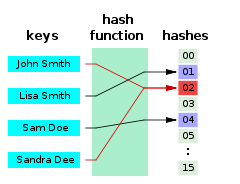
\includegraphics[scale=0.7]{img/collision.png}
\caption{In this diagram, the hash function returns the same index for both John Smith and Sandra Dee.  This is a collision.}
\end{figure}

\subsection{Designing to avoid collisions}
Hash tables are made very large to avoid collisions.  If we have a table of size $n$, and we want to store more than $n$ elements, then we will definitely have a collision somewhere.  This is called the pidgeonhole principle: remember this, because it can make CS240, the theory of computation, much easier.

Hash functions are also specially designed to spread things evenly.  I'm not entirely sure how this is done, as it obviously requires knowing something about the data beforehand.

Fun fact: the Java String hash function is:
\[
h(s) = \sum_{i=0}^{n-1} s[i] * 31^{n-1-i}
\]
where $s$ is the string, $n$ is its length, and $h$ is the hash function.

Note that 31 is a prime number.  This may or may not be significant.  We have to modulo this to get an actual index.

\subsection{Resolution}

Resolving collisions inevitably hurts the performance of hash tables.  Some resolution methods reduce lookup speeds to be $O(n)$, but with much more time and space overhead than a standard array.

\subsubsection{Open addressing}
Open addressing is a common method to resolve collisions - the idea is to find a new address for the new object $o$.  However, as the percentage of elements in the table (called the \textit{load factor} increases, finding empty space can be extremely difficult.

The new address is found by \textit{probing}; this process depends on a constant value $i$, and $k$, which begins at 0 and is incremented until an open address is found.  Some common probing sequences:
\begin{enumerate}
\item Linear probing - address is the original plus $ik$.
\item Quadratic probing - address is original plus $(ik)^2$. 
\item Double hashing - address is original plus $k*f(o)$, where $f(o)$ is a second hash function.
\end{enumerate}

Double hashing can be computationally expensive, and linear probing doesn't perform well when things cluster together.  Quadratic probing is somewhere in between.  All open addressing methods do not perform well under high load factors.

\subsubsection{Chaining}
In a chaining hash table, entries are actually linked lists.  When a collision occurs, the new element is simply appended to the linked list.  Performance degrades more gracefully with load factor in a chaining scheme.  
In the worst case, the hash table degenerates into one linked list.

\begin{figure}
\centering
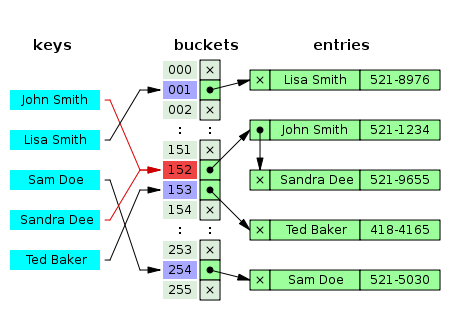
\includegraphics[scale=0.7]{img/chaining.png}
\caption{Hash table with chaining, using linked lists.}
\end{figure}

\subsubsection{Rehashing}
Another alternative is to create a whole new hash table or use a different hash function, and rehash all existing entries.  The high cost makes it overkill for a single collision, but in some situations, e.g. when the load factor gets too high, this is an appropriate response.

\section{Weaknesses}
\subsection{Removal}
Removal is straightforward for chaining hash tables: just remove an item from the appropriate linked list.  But what about probing hash tables?  In probing schemes, probing continues until an empty space is found - if an element is removed in the middle of a probing sequence, then every element after it is no longer accessible by the original hash.

Consider linear probing.  How to remove an element in the middle of a collision chain?  Putting an empty space in the middle of the chain breaks the chain.  All elements afterwards are not accessible afterwards.

It may be possible to remove the element and replace it with another in the collision chain.  However, in a scheme such as quadratic probing, we may not know which chains the element belongs to.

The simple solution to this is to \textit{lazy delete} the node, marking it as deleted but still occupied.  That way, the chain is not broken, but the element is not accessible.  Of course, this wastes memory.

\subsection{Degenerate performance}
Degrading into $O(n)$ performance might seem pretty good, but it's not when you expect much faster performance.  There is overhead for the hash table itself, the key objects, the value objects, and the number of slots in a hash table is generally generally more (1.3 to 2 times) than the number of elements stored.

Many scripting languages use chaining hash tables with simple, deterministic hashes.  Many scripting languages are also used to program web applications.  Putting the two together, hackers have found a simple way to mount a denial-of-service attack on most web applications.\footnote{The paper title is \textit{Effective DoS Attacks Against Web Application Platforms.}}

Attackers know what hash functions are used, so with a little reverse engineering, they can send data which all hash to the same location.  This can hang up most web servers.

The solution, at least for Python, was to change the hash function randomly for each running instance, so that the hash function cannot be reverse engineered.

\subsection{Query limitations}
The speed of hash tables potentially makes them useful for database indices, but only for certain types of data.  You can't perform range queries on hash tables, e.g. get all integers between 1 and 100, because there is no concept of order in a hash table.  Thus, B-trees are more often used for databases.

\section{Examples}
\begin{problem}
{Given a string, find the first character which only occurs once.  For example, return 'a' for the input 'bbadfgchcbc'.}
\end{problem}

There is a simple $O(n^2)$ solution where, on encountering a character, we check every other character in the string for equality.  There are many ways to speed this up, but will still lead to an $O(n^2)$ solution.

We can use a hash table which maps characters to integers.
\begin{enumerate}
\item We go through every character of the string, hashing each character, and incrementing the corresponding index.
\item We go through every character a second time, and find the first character whose indexed value is 1.
\end{enumerate}
This is an O(n) solution.

\begin{problem}
{Given an English word in the form of a string, find all valid anagrams for that string quickly.  Assume you have access to all words, can pre-compute anything you want, and can store it.}
\end{problem}

There is a solution which involves testing all permutations of the string for membership in a hash table.  This is perhaps more obvious, but slow.

A chaining hash table is more natural.  Use it in the following way:
\begin{enumerate}
\item Iterate over every word in English.
\item Sort the characters in alphabetical order and use that as a key.
\item Place the word in the appropriate index.
\end{enumerate}

If there are no collisions (big if!), then each bin will contain a linked list with all valid words using a given set of characters.  Otherwise, you will still have some sorting out to do.

\begin{problem}
{Given an array of integers, and a target integer, find two numbers in the array which add up to the target integer.}
\end{problem}

Let's say our target integer is $j$.  The obvious solution is to double loop through the array and see if the sum of two numbers is $j$.  This is $O(n^2)$.

We can use a hash table (surprise) to achieve $O(n)$ performance:
\begin{enumerate}
\item Loop through the array once, storing each number in a hash table.
\item Loop through the array again.  For each integer $i$, check to see if $j-i$ is in the table.  If so, return $i$ and $j-i$.
\end{enumerate}

\end{document}
